\documentclass[12pt, twoside]{article}
\documentclass[12pt, twoside]{article}
\usepackage[letterpaper, margin=1in, headsep=0.2in]{geometry}
\setlength{\headheight}{0.6in}
%\usepackage[english]{babel}
\usepackage[utf8]{inputenc}
\usepackage{microtype}
\usepackage{amsmath}
\usepackage{amssymb}
%\usepackage{amsfonts}
\usepackage{siunitx} %units in math. eg 20\milli\meter
\usepackage{yhmath} % for arcs, overparenth command
\usepackage{tikz} %graphics
\usetikzlibrary{quotes, angles}
\usepackage{graphicx} %consider setting \graphicspath{{images/}}
\usepackage{parskip} %no paragraph indent
\usepackage{enumitem}
\usepackage{multicol}
\usepackage{venndiagram}

\usepackage{fancyhdr}
\pagestyle{fancy}
\fancyhf{}
\renewcommand{\headrulewidth}{0pt} % disable the underline of the header
\raggedbottom
\hfuzz=2mm %suppresses overfull box warnings

\usepackage{hyperref}

\fancyhead[LE]{\thepage}
\fancyhead[RO]{\thepage \\ First and last name: \hspace{2.5cm} \,\\ Section: \hspace{2.5cm} \,}
\fancyhead[LO]{BECA/Huson/Geometry: Construction \\* 2 October 2024}

\begin{document}

\subsubsection*{1.19 Classwork: Rotation, translation, \& reflection \hfill CCSS.HSG.CO.A.5}
\begin{enumerate}
  \item Rotate $\triangle JKL$ counterclockwise $90^\circ$ around the origin, labeling the image $\triangle J'K'L'$.
  \begin{center}
      \begin{tikzpicture}[scale=.6]
      \draw [<->] (-6.4,0)--(6.4,0) node [right] {$x$};
      \draw [<->] (0,-5.4)--(0,5.4) node [above] {$y$};
      \foreach \x in {-4,4}
        \draw[shift={(\x,0)},color=black] (0pt,-5pt) -- (0pt,5pt) node[below=5pt]  {$\x$};
      \foreach \y in {-4,4}
        \draw[shift={(0,\y)},color=black] (-5pt,0pt) -- (5pt,0pt) node[right=5pt]  {$\y$}; 
      \draw [thick]
        (0,0) node[below right] {$J$}--
        (4,4) node[right] {$K(4,4)$}--
        (4,0) node[above right] {$L$}--cycle;  
    \end{tikzpicture}
  \end{center}
  
  \item On the axes below, mark and label the origin, $O(0,0)$. Plot the point $P(4,1)$ and segment $\overline{OP}$. Graph its image, $\overline{O'P'}$, after a $90^\circ$ counterclockwise rotation around the origin. Mark $P'$ and write it down as a coordinate pair.
    \begin{center}
      \begin{tikzpicture}[scale=1]
      \draw [help lines] (-5,-5) grid (5,5);
      \draw [thick, <->] (-5.4,0) -- (5.4,0) node [right] {$x$};
      \draw [thick, <->] (0,-5.4)--(0,5.4) node [above] {$y$};
      \foreach \x in {-5,...,-1,1,2,3,4,5}
        \draw[shift={(\x,0)},color=black] (0pt,-3pt) -- (0pt,3pt) node[below=5pt]  {$\x$};
      \foreach \y in {-5,...,-1,1,2,3,4,5}
        \draw[shift={(0,\y)},color=black] (-3pt,0pt) -- (3pt,0pt) node[left=5pt]  {$\y$}; 
    \end{tikzpicture}
  \end{center}

\newpage
\item A rotation maps triangle $DEF$ onto triangle $LMN$. \\[0.5cm]
Write the letter or letters for each corresponding object. \vspace{0.5cm}
    \begin{multicols}{2}
      \begin{tikzpicture}[scale=1]
        \coordinate [label=above left:$L$](A) at (85:2);
        \coordinate [label=above left:$M$](B) at (0, 0);
        \coordinate [label=right:$N$](C) at (25:3.5);
        \draw [thick] (A)--(B)--(C)--cycle;
        \draw [thick, rotate=-90] (85:2) node[right]{$D$}--
        (0,0) node[below left]{$E$}--
        (25:3.5) node[right]{$F$}--cycle;
      \end{tikzpicture}

      \begin{enumerate}
        \item $E \rightarrow$ \vspace{1.5cm}
        \item $F \rightarrow$ \vspace{1.5cm}
        \item $\overline{DF} \rightarrow$ \vspace{1.5cm}
      \end{enumerate}
    \end{multicols}

\item A rotation centered at the origin maps $A$ to $A'$, as shown, $A(3,1) \rightarrow A'(-1,3)$.
\begin{multicols}{2}
  \begin{enumerate}
    \item Identify the rotation:
    \begin{enumerate}[label=(\Alph*)]
      \item Clockwise $180^\circ$
      \item Counter clockwise $180^\circ$
      \item Clockwise $90^\circ$
      \item Counter clockwise $90^\circ$
      \item None of the above
    \end{enumerate} \vspace{1cm}
    \item Apply the same translation to $C(5,1)\rightarrow C'(x,y)$. Plot and label the point $C'$ as an ordered pair.
    \end{enumerate}
    \begin{flushright}
    \begin{tikzpicture}[scale=0.7]
      \draw [help lines] (-3,-3) grid (7,7);
      \draw [thick, ->] (-3.2,0) -- (7.4,0) node [below right] {$x$};
      \draw [thick, ->] (0,-3.2)--(0,7.4) node [left] {$y$};
      \draw [fill] (3,1) circle [radius=0.1] node[below] {$A(3,1)$};
      \draw [fill] (-1,3) circle [radius=0.1] node[below left] {$A'(-1,3)$};
      \draw [fill] (5,1) circle [radius=0.1] node[right] {$C(5,1)$};
    \end{tikzpicture}
    \end{flushright}
\end{multicols}

\newpage
\item On the axes below, plot the point $A(-4,-1)$ and its image, $A'$, after the translation $(x,y) \rightarrow (x+6,y-3)$. Label the image as a coordinate pair.
    \begin{center}
      \begin{tikzpicture}[scale=.48]
      \draw [help lines] (-5,-5) grid (5,5);
      \draw [thick, <->] (-5.4,0) -- (5.4,0) node [right] {$x$};
      \draw [thick, <->] (0,-5.4)--(0,5.4) node [above] {$y$};   
    \end{tikzpicture}
  \end{center}

\item The image of triangle $ABC$ after a translation is $\triangle A'B'C'$. Is the area of the triangle greater, smaller, or the same after the translation? Justify your answer. \vspace{4cm}

\item Find the result after the point $B(-2,5)$ is translated first to the right five and down one, and then by a second translation to the right one and down three. \par 
Use proper notation and show all three points--$B$, $B'$, and $B''$--as ordered pairs. \vspace{3cm}

\item What translation would map $P(4,7)\rightarrow P'(6,2)$?

\newpage
\item Reflect the point $A(4)$ across the origin. (flip the number line) Mark and label it $A'$.
  \begin{center}
      \begin{tikzpicture}
        \draw [<->] (-7.5,0)--(7.5,0);
        \foreach \x in {-7,...,7}
          \draw[shift={(\x,0)},color=black] (0pt,-3pt) -- (0pt,3pt) node[below=5pt]  {$\x$};
          \draw [fill] (4,0) circle [radius=0.05] node[above] {$A(4)$};
      \end{tikzpicture}
    \end{center}

  \item On the axes below, graph the point $P(-4,3)$ and its image, $P'$, after a reflection across the $x$-axis. Mark $P'$ and write it down as a coordinate pair.
    \begin{center}
      \begin{tikzpicture}[scale=.6]
      \draw [help lines] (-5,-5) grid (5,5);
      \draw [thick, <->] (-5.4,0) -- (5.4,0) node [right] {$x$};
      \draw [thick, <->] (0,-5.4)--(0,5.4) node [above] {$y$};
      \foreach \x in {-5,...,-1,1,2,3,4,5}
        \draw[shift={(\x,0)},color=black] (0pt,-3pt) -- (0pt,3pt) node[below=5pt]  {$\x$};
      \foreach \y in {-5,...,-1,1,2,3,4,5}
        \draw[shift={(0,\y)},color=black] (-3pt,0pt) -- (3pt,0pt) node[left=5pt]  {$\y$}; 
    \end{tikzpicture}
  \end{center}

\item A reflection maps $Q(4,3)$ onto $Q'(4,-3)$. Is the reflection across the $x$-axis or the $y$-axis? \vspace{1cm}

\item Reflect $\triangle JKL$ across the $y$-axis, labeling the image $\triangle J'K'L'$.
\begin{center}
    \begin{tikzpicture}[scale=.48]
    \draw [help lines] (-8,-6) grid (8,6);
    \draw [thick, <->] (-8.4,0) -- (8.4,0) node [right] {$x$};
    \draw [thick, <->] (0,-6.4)--(0,6.4) node [above] {$y$};  
    \draw [thick]
      (4,3) node[above right] {$J$}--
      (2,-3) node[below] {$K$}--
      (6,0) node[below right] {$L$}--cycle;  
  \end{tikzpicture}
\end{center}

\newpage
\item Triangle $A'B'C'$ is the image of triangle $ABC$ after a reflection. Is triangle $ABC$ congruent to $A'B'C'$? Explain why. \vspace{3cm}

\item In the graph below, a transformation maps $\triangle PQR$ onto $\triangle STU$.
\begin{multicols}{2}
  \begin{enumerate}
    \item Completely identify the transformation.
    \item What point corresponds to $T$?
    \item Is $R$ the image of $U$, or its preimage? \vspace{1cm}
  \end{enumerate}
    \begin{tikzpicture}[scale=.6]
    \draw [help lines] (-6,-4) grid (6,7);
    \draw [thick, <->] (-6.4,0) -- (6.4,0) node [right] {$x$};
    \draw [thick, <->] (0,-4.4)--(0,7.4) node [above] {$y$};  
    \draw [thick]
      (-1,5) node[above] {$P$}--
      (-4,4) node[left] {$Q$}--
      (-2,1) node[below left] {$R$}--cycle;
    \draw [thick]
    (1,5) node[above] {$S$}--
    (4,4) node[above] {$T$}--
    (2,1) node[below right] {$U$}--cycle;
  \end{tikzpicture}
\end{multicols}

\item In the graph below, a transformation maps $\triangle ABC \rightarrow \triangle A'B'C'$.
\begin{multicols}{2}
Angie says the triangle must have been reflected across the $y$-axis. Robbie says it might have been reflected, but it could also have been translated to the right.\\[0.25cm] 
Who is correct? Justify your answer.
    \begin{tikzpicture}[scale=.6]
    \draw [help lines] (-6,-4) grid (6,7);
    \draw [thick, <->] (-6.4,0) -- (6.4,0) node [right] {$x$};
    \draw [thick, <->] (0,-4.4)--(0,7.4) node [above] {$y$};  
    \draw [thick]
      (-2,5) node[above] {$A$}--
      (-3,1) node[below] {$B$}--
      (-1,1) node[below] {$C$}--cycle;
    \draw [thick]
    (2,5) node[above] {$A'$}--
    (3,1) node[below] {$B'$}--
    (1,1) node[below] {$C'$}--cycle;
  \end{tikzpicture}
\end{multicols}

\newpage
\item Rotate the triangle $90^\circ$ clockwise around the origin, $\triangle ABC \rightarrow \triangle A'B'C'$. Complete the table of the coordinates and plot and label the image on the grid. \vspace{0.5cm}
\begin{multicols}{2}
  $A(1,2) \rightarrow$ \\[0.7cm]
  $B(1,4) \rightarrow$ \\[0.7cm]
  $C(4,2) \rightarrow$ \\[0.7cm]
    \begin{tikzpicture}[scale=.75]
    \draw [help lines] (-5,-5) grid (5,5);
    \draw [thick, <->] (-5.4,0) -- (5.4,0) node [right] {$x$};
    \draw [thick, <->] (0,-5.4)--(0,5.4) node [above] {$y$};  
    \draw [thick]
      (1,2) node[below left] {$A$}--
      (1,4) node[above left] {$B$}--
      (4,2) node[below] {$C$}--cycle;  
    \end{tikzpicture}
  \end{multicols}

\item $\triangle ABC$ is shown with vertices $A(-1,2)$, $B(6,1)$, and $C(5,4)$. Rotate the triangle $90^\circ$ counter clockwise around the origin. Write down its coordinates in a table and plot and label it on the graph.
  \begin{flushright}
    \begin{tikzpicture}[scale=0.7]
      \draw [help lines] (-7,-5) grid (7,7);
      \draw [thick, <->] (-7.4,0) -- (7.4,0) node [below right] {$x$};
      \draw [thick, <->] (0,-5.4)--(0,7.4) node [left] {$y$};
      \draw [thick] (-1,2) node[below] {$A$}--
        (6,1) node[right] {$B$}--
        (5,4) node[above right] {$C$}--
        cycle;
    \end{tikzpicture}
    \end{flushright}

\newpage
  \item Given $\triangle WIN \cong \triangle W'I'N'$. Describe the rigid motion mapping $\triangle WIN \rightarrow \triangle W'I'N'$.
  \begin{flushright}
    \begin{tikzpicture}[scale=.48]
      %\draw [help lines] (-10,-7) grid (10,7);
      \draw [thick, <->] (-5.4,0) -- (5.4,0) node [right] {$x$};
      \draw [thick, <->] (0,-4.4)--(0,4.4) node [above] {$y$};  
      \draw [thick]
      (1,0) node[above] {$W$}--
      (4,3) node[right] {$I$}--
      (4,-3) node[below right] {$N$}--cycle;
      \draw [thick]
      (-1,0) node[below] {$W'$}--
      (-4,3) node[left] {$N'$}--
      (-4,-3) node[below left] {$I'$}--cycle;
    \end{tikzpicture}
  \end{flushright}

  \item Determine and state the sequence of transformations applied to map $BECA$ to $B''E''C''A''$.
  \begin{flushright}
      \begin{tikzpicture}[scale=.48]
      \draw [help lines] (-8,-6) grid (10,6);
      \draw [thick, <->] (-8.4,0) -- (10.4,0) node [right] {$x$};
      \draw [thick, <->] (0,-6.4)--(0,6.4) node [above] {$y$};  
      \draw [thick]
        (3,1) node[left] {$B$}--
        (3,5) node[above] {$E$}--
        (7,4) node[above] {$C$}--
        (7,2) node[right] {$A$}--cycle;
      \draw [thick]
        (-3,-1) node[left] {$B''$}--
        (-3,-5) node[left] {$E''$}--
        (1,-4) node[right] {$C''$}--
        (1,-2) node[right] {$A''$}--cycle; 
    \end{tikzpicture}
  \end{flushright}

  \item Determine and state the transformation mapping $\triangle NOP$ onto $\triangle QRP$. 
    \begin{flushright}
        \begin{tikzpicture}[scale=.48]
        \draw [help lines] (-7,-5) grid (7,7);
        \draw [thick, <->] (-7.4,0) -- (7.4,0) node [right] {$x$};
        \draw [thick, <->] (0,-5.4)--(0,7.4) node [above] {$y$};  
        \draw [thick]
          (-1,5) node[above] {$N$}--
          (-4,4) node[left] {$O$}--
          (1,1) --cycle;
        \draw [thick]
        (3,-3) node[below] {$Q$}--
        (6,-2) node[above right] {$R$}--
        (1,1) node[above right] {$P$}--cycle;
      \end{tikzpicture}
    \end{flushright}


\end{enumerate}
\end{document}